% !TeX TXS-program:compile = txs:///pdflatex/[--shell-escape]

\documentclass[10pt,  english, makeidx, a4paper, titlepage, oneside]{book}
\usepackage{babel}
\usepackage{fancyhdr}
\usepackage{makeidx}
\usepackage{titlesec}
\usepackage{listings}
\usepackage{booktabs}

\newenvironment{listato}{\footnotesize}{\normalsize }

%\pagestyle{empty}

\textwidth 15.5cm
\textheight 23cm
\topmargin -1cm
\oddsidemargin -0.5cm
\linespread{1.1}

\pagestyle{fancy}
\lhead{}
\chead{Microelectronic Systems}
\lfoot{}
\cfoot{}
\rfoot{}
\rhead{\thepage}

\usepackage{graphicx}
\usepackage{amsmath}
\usepackage{amsfonts}
\usepackage{amsthm}
\usepackage{amssymb}
%\oddsidemargin -1.1cm
\usepackage{graphicx}
\usepackage{caption}
\usepackage{float}
\usepackage{amsmath}
\usepackage{amssymb}
\usepackage{amsfonts}
\usepackage{amsthm}
%\usepackage{subscript}
\usepackage{empheq}
\usepackage{verbatim}
\usepackage{fancyvrb}
\usepackage{hyperref}

% Code packages
\usepackage{listings}
\usepackage{minted}
\usepackage{tikz}
\usepackage{bytefield}
\usepackage{xparse}
\usepackage{etoolbox}

% For circuit diagrams
\usepackage[siunitx, RPvoltages]{circuitikz}
\usepackage{amsmath,amsbsy,amsfonts,amssymb}
\usepackage[per-mode=symbol]{siunitx}
\usepackage{steinmetz}
\usepackage[utf8]{inputenc}
%\usepackage[T1]{fontenc}

\newcommand{\micro}{\ensuremath{\mu}}
\newcommand{\phasorName}[1]{ \ensuremath{ \boldsymbol{\hat #1} } }
\newcommand{\impedance}[1]{ \ensuremath{ \boldsymbol{#1} } }
\newcommand{\complexPol}[2]{\ensuremath{#1\phase{#2}}}
\newcommand{\complexPolDeg}[2]{\ensuremath{#1\phase{#2\degree}}}

% new units
\DeclareSIUnit{\Vef}{\volt_{ef}} % volt eficaz
\DeclareSIUnit{\Vrms}{\volt_{rms}} % volt RMS
\DeclareSIUnit{\Vpp}{\volt_{pp}} % volt peak-to-peak

\DeclareSIUnit{\Aef}{\ampere_{ef}} % ampere eficaz
\DeclareSIUnit{\Arms}{\ampere_{rms}} % ampere rms
\DeclareSIUnit{\App}{\ampere_{pp}} % ampere peak-to-peak

% logic Commands
\newcommand{\NOT}[1]{\ensuremath{\overline{\mbox{\ensuremath{#1}}}}}
\newcommand{\AND}{\ensuremath{\cdot}}
\newcommand{\OR}{\ensuremath{+}}
\newcommand{\XOR}{\ensuremath{\oplus}}
\newcommand{\XNOR}{\ensuremath{\odot}}

\newtoggle{newarg}
\toggletrue{newarg}
\newcounter{bitfieldsize}
\usetikzlibrary{positioning}
\usetikzlibrary{decorations.pathreplacing}

\newcommand\mybitbox[1] {% <- here
    \iftoggle{newarg}{% <- here
        \setcounter{bitfieldsize}{ #1 }% <- here
        \togglefalse{newarg}% <- here
    }{% <- here
        \bitbox{\value{bitfieldsize}}{#1}% <- here
        \toggletrue{newarg}% <- here
    }}

\NewDocumentCommand\bitboxlist {  >{\SplitList{;}}m} {% <- here
    \ProcessList{#1}{\mybitbox}}

\newcounter{instsize}
\NewDocumentCommand\mybytefield{m >{\SplitList{;}}m} {% <- here
    \setcounter{instsize}{#1 - 1 }% <- here
    \begin{figure}[htbp]
        \begin{center}
            \begin{bytefield}[endianness=big,bitwidth=1em]{#1}
                \bitheader{0-\value{instsize}} \\
                \ProcessList{#2}{\bitboxlist}% <- here
            \end{bytefield}
        \end{center}
    \end{figure}}

\newcommand\staticbitbox[4] {% <- here
    \bitbox{#1}{#2} \bitbox{#3}{#4}}


\newcommand\MemoryLayout[1]{
  \begin{tikzpicture}[scale=0.3]
     \draw[thick](0,0)--++(0,3)node[above]{$0$};
     \foreach \pt/\col/\lab [remember=\pt as \tp (initially 0)] in {#1} {
       \foreach \a in {\tp,...,\pt-1} {
          \draw[fill=\col](-\a,0) rectangle ++(-1,2);
       }
       \draw[thick](-\pt,0)--++(0,3)node[above]{$\pt$};
       \if\lab\relax\relax\else
         \draw[thick,decorate, decoration={brace,amplitude=4mm}]
            (-\tp,-0.2)--node[below=4mm]{\lab} (-\pt,-0.2);
       \fi
     }
  \end{tikzpicture}
}

\NewDocumentCommand{\codeword}{v}{%
\texttt{\textcolor{blue}{#1}}%
}



\newcommand\memsection[4]{
\bytefieldsetup{bitheight=#3\baselineskip}    % define the height of the memsection
\bitbox[]{10}{
\texttt{#1}     % print end address
\\ \vspace{#3\baselineskip} \vspace{-2\baselineskip} \vspace{-#3pt} % do some spacing
\texttt{#2} % print start address
}
\bitbox{16}{#4} % print box with caption
}

\lstdefinelanguage{VHDL}{morekeywords={library,use,all,entity,generic, is,port,in,out,end,architecture,of,begin,and,if,then,else,elsif,process},morecomment=[l]--}

\lstdefinestyle{vhdl}{language = VHDL, basicstyle = \ttfamily, keywordstyle = \color{keyword}\bfseries, commentstyle = \color{comment}}

\titleformat{\chapter}[display]
{\normalfont\Large\filcenter\sffamily}
{\titlerule[0.5pt]%
\vspace{1pt}
\titlerule
\vspace{1pc}
\LARGE\MakeUppercase{\chaptertitlename} \thechapter
}
{1pc}
{\titlerule
\vspace{1pc}
\Huge}

\makeindex

\begin{document}

\frontmatter
\begin{titlepage}
\vspace{0cm}
\centerline{

\includegraphics[width=0.6\textwidth]{./polito_logo.jpg}} 
\vspace{0.5cm}
\centerline{\huge\sf QEMU implementation of NXP S32K3X8EVB board}
\vspace{1cm}
\centerline{\Huge\sf Group 10}
\bigskip
\centerline{\huge\sf Project Report}
\vspace{1cm}
\centerline{\Large Master degree in Computer Engineering: Embedded Systems}
\vspace{2.5cm}
%%%%%%%%%%%%%%%%%%%%%%%%%%%%%%%%%%%%%%%%%%%%%%%%%%%%%%
%
{\large Referents:}

Prof. Stefano Di Carlo

Prof. Carpegna Alessio 

Prof. Carpegna Alessio

Prof. Eftekhari Moghadam Vahid

Prof. Magliano Enrico


\bigskip
\vspace{1cm}
%
%%%%%%%%%%%%%%%%%%%%%%%%%%%%%%%%%%%%%%%%%%%%%%%%%%%%%%
%
{\large Authors:}
% \bigskip
%
%%%%%%%%%%%%%%%%%%%%%%%%%%%%%%%%%%%%%%%%%%%%%%%%%%%%%%
% AUTHORS
% Change the name of the Group participants here
%

Francesco Mignone

Leonardo Gallina 

Andrea Baraldi

Silvia Bonenti

Lorenzo Parata
%
%%%%%%%%%%%%%%%%%%%%%%%%%%%%%%%%%%%%%%%%%%%%%%%%%%%%%%
\begin{center}
    % {\large \today}
\end{center}
\end{titlepage}

% Abstract on the report fot the NXP S32K3X8EVB board on QEMU
\chapter{Abstract}
\label{Abstract}

This report presents the development and implementation of a simulation environment for the NXP S32K3X8EVB board using QEMU. The primary objective of this project is to facilitate the testing and development of embedded software applications without the need for physical hardware, thereby reducing costs and increasing accessibility for developers.
The report begins with an overview of the NXP S32K3X8EVB board, highlighting its key features and specifications. It then delves into the architecture and capabilities of QEMU, emphasizing its suitability for simulating embedded systems. The core of the report focuses on the step-by-step process of setting up the QEMU environment to emulate the S32K3X8EVB board, including the configuration of necessary peripherals and interfaces (UART and SPI).
Furthermore, the report discusses the challenges encountered during the implementation phase and the solutions devised to overcome them.

Finally, the report concludes with an evaluation of the simulation environment's performance and its potential applications in embedded systems development. The successful implementation of this project demonstrates the feasibility of using QEMU for simulating complex embedded systems, paving the way for future advancements in this field.
The report is structured to provide a comprehensive understanding of the project, making it a valuable resource for developers and researchers interested in embedded systems simulation. The structure is as follows:
\begin{itemize}
    \item Chapter 1: Introduction - Provides background information and outlines the objectives of the project.
    \item Chapter 2: NXP S32K3X8EVB Board Overview - Details the specifications and features of the board.
    \item Chapter 3: QEMU Overview - Discusses the architecture and capabilities of QEMU.
    \item Chapter 4: Implementation - Describes the step-by-step process of setting up the simulation environment.
    \item Chapter 5: FreeRTOS Porting - Explains the process of porting FreeRTOS to the simulated environment.
    \item Chapter 6: Testing and Conclusion - Evaluates the performance of the simulation environment and summarizes key findings.
    \item References - Lists the sources and references used throughout the report.
    \item Appendices - Includes supplementary material such as code snippets and configuration files.
\end{itemize} 

A prior knowledge of embedded systems, real-time operating systems, transmission protocols and virtualization technologies is beneficial for understanding the content of this report.

\tableofcontents

\mainmatter
%%%%%%%%%%%%%%%%%%%%%%%%%%%%%%%%%%%%%%%%%%%%%%%%%%%%%%
%    
%
\chapter{Introduction}

\section{Project Objectives}

The goal of this project is to create a simulation environment for the NXP S32K3X8EVB board using QEMU. This environment will allow developers to test and develop embedded software applications without the need for physical hardware, thereby reducing costs and increasing accessibility. The specific objectives of the project include:
\begin{itemize}
    \item Setting up QEMU to emulate the NXP S32K3X8EVB board.
    \item Configuring necessary peripherals and interfaces, such as UART and SPI, to ensure accurate simulation of the board's functionality.
    \item Porting FreeRTOS to the simulated environment to enable real-time operating system capabilities.
    \item Testing the simulation environment with sample applications to validate the implementation.
    \item Documenting the implementation process, challenges encountered, and solutions devised to overcome them.
\end{itemize}

In particular the pheripherals that will be implemented are:
\begin{itemize}
    \item UART (Universal Asynchronous Receiver/Transmitter)
    \item SPI (Serial Peripheral Interface)
\end{itemize}

\section{Tools and Technologies}

\subsection{NXP S32K3X8EVB Board}

The NXP S32K3X8EVB board is a development platform designed for automotive and industrial applications. It is based on the S32K3 series of microcontrollers, which feature an ARM Cortex-M7 core. The board includes various peripherals, such as UART, SPI, I2C, ADC, and GPIOs, allowing developers to interface with external devices and sensors. The S32K3X8EVB board is widely used in the automotive industry for applications such as motor control, body electronics, and sensor fusion.

\subsection{QEMU}

QEMU (Quick Emulator) is an open-source machine emulator and virtualizer that allows users to run operating systems and applications for one machine on a different machine. It supports a wide range of architectures, including ARM, x86, MIPS, and PowerPC, making it a versatile tool for simulating various hardware platforms.
QEMU operates in two primary modes: full system emulation and user-mode emulation. In full system emulation, QEMU emulates an entire hardware platform, including the CPU, memory, and peripherals, allowing users to run complete operating systems. In user-mode emulation, QEMU can run applications compiled for one architecture on another architecture by translating system calls and library functions.
QEMU's flexibility and extensibility make it an ideal choice for simulating embedded systems. It provides a rich set of features, including support for various peripherals, networking capabilities, and the ability to create custom device models. Additionally, QEMU's open-source nature allows developers to modify and extend its functionality to suit their specific needs.

\subsection{FreeRTOS}
FreeRTOS is an open-source real-time operating system (RTOS) designed for embedded systems. It provides a lightweight and efficient kernel that enables multitasking, inter-task communication, and resource management. FreeRTOS is widely used in various applications, including automotive, industrial, and consumer electronics, due to its simplicity, portability, and scalability.
It offers a rich set of features, such as task scheduling, semaphores, queues, and timers, allowing developers to create complex real-time applications with ease. FreeRTOS is also highly configurable, enabling users to tailor the kernel to their specific requirements by selecting only the necessary components.

\subsection{Development Environment}
The development environment for this project includes a combination of software tools and libraries to facilitate the implementation and testing of the simulation environment. Key components of the development environment include:
\begin{itemize}
    \item \textbf{QEMU}: The primary tool for emulating the NXP S32K3X8EVB board. The vesion used in this project is QEMU 9.0.0.
    \item \textbf{NXP Toolchain}: A collection of compilers and tools for building embedded applications, including the ARM GCC compiler for compiling code for the ARM Cortex-M7 architecture provided by NXP.
    \item \textbf{FreeRTOS Source Code}: The source code for FreeRTOS, which will be ported to the simulated environment.
    \item \textbf{Debugging Tools}: Tools such as GDB (GNU Debugger) for debugging and testing the simulation environment.
    \item \textbf{Version Control System}: Git is used for managing the source code and tracking changes throughout the development process.
\end{itemize}

\section{Project Structure}
The project is organized into several key components, each responsible for a specific aspect of the simulation environment. The main components include:


\begin{forest}
    for tree={
        font=\ttfamily,
        grow'=0,
        child anchor=west,
        parent anchor=south,
        anchor=west,
        calign=first,
        inner xsep=7pt,
        edge path={
          \noexpand\path [draw, \forestoption{edge}]
          (!u.south west) +(7.5pt,0) |- (.child anchor) pic {folder} \forestoption{edge label};
        },
        % style file node 
        file/.style={edge path={\noexpand\path [draw, \forestoption{edge}]
          (!u.south west) +(7.5pt,0) |- (.child anchor) \forestoption{edge label};},
          inner xsep=2pt,font=\small\ttfamily
                     },
        before typesetting nodes={
          if n=1
            {insert before={[,phantom]}}
            {}
        },
        fit=band,
        before computing xy={l=15pt},
      }  
  [group10
    [qemu
      [hw
        [arm
            [S32K3X8EVB.c - Board implementation file, file]
            [S32K3X8EVB\_MCU.c - MCU implementation file, file]
        ]
        [char
            [S32K3X8EVB\_UART.c - UART implementation file, file]
        ]
        [ssi
            [S32K3X8EVB\_SPI.c - SPI implementation file, file]
        ]
      ]
      [include
        [arm
            [S32K3X8EVB.h - Board header file, file]
            [S32K3X8EVB\_MCU.h - MCU header file, file]
        ]
        [char
            [S32K3X8EVB\_UART.h - UART header file, file]
        ]
        [ssi
            [S32K3X8EVB\_SPI.h - SPI header file, file]
        ]
      ]
    ]
    [FreeRTOS\_App - FreeRTOS application
      [main.c - Main application file, file]
      [FreeRTOSConfig.h - FreeRTOS configuration file, file]
      [pheripherals.c - Function for the pheripherals, file]
      [pheripherals.h - Header file for the pheripherals, file]
      [Makefile - Build file, file]
    ]
    [gcc-10.2.0-Earmv7GCC-eabi - NXP toolchain
    ]
    [material
      [S32K3.pdf - MCU reference manual, file]
      [S32K3X8EVB-Q289HWUM.pdf - Board user manual, file]
      [S32K3xx\_memory\_map.xls - Memory and Pheripheral map, file]
    ]
    [Docs
      [Source
        [report - Source files for the report]
        [presentation - Source files for the presentation]
        [Group10\_Presentation.pdf, file]
        [Group10\_Report.pdf, file]
      ]
    ]
    [qemu\_old - QEMU version 9.0.42 (not complaint to our implementation)]
  ]
\end{forest}


% \section{NXP S32K3X8EVB Board Overview}

The S32K3X8EVB-Q289 is an evaluation and development board for general-purpose automotive and industrial applications.
Based on the 32-bit Arm Cortex-M7 S32K3 MCU in a 289 MAPBGA package, the S32K3X8EVB-Q289 offers a multicore mode, Hardware Security Engine (HSE), Over-the-Air (OTA) support, advanced connectivity and low power.
The S32K3X8EVB-Q289 board is designed to support a wide range of applications, including motor control, body electronics, and sensor fusion. It features a variety of peripherals and interfaces, such as UART, SPI, I2C, ADC, and GPIOs, allowing developers to interface with external devices and sensors. 

\begin{figure}[H]
    \centering
    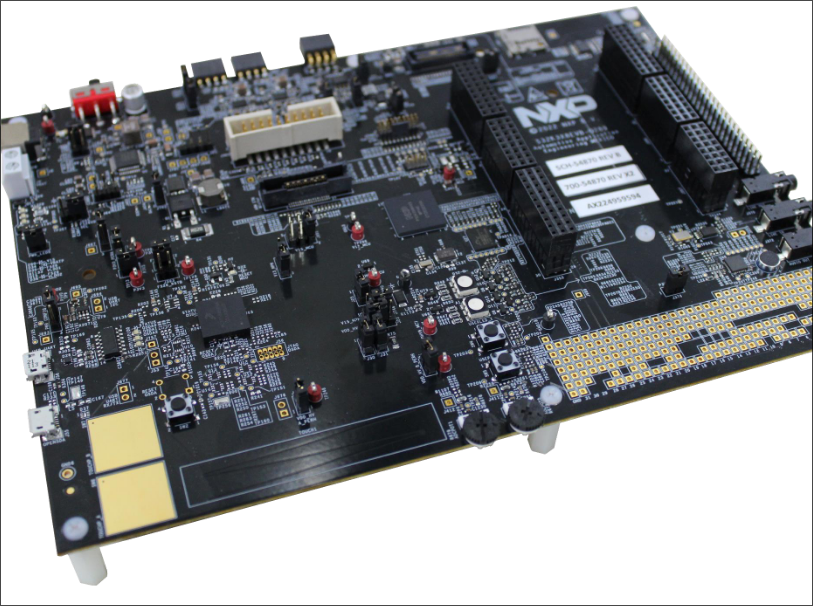
\includegraphics[width=0.7\textwidth]{chapters/figures/Board.png}
    \caption{NXP S32K3X8EVB Board}
    \label{fig:s32k3x8evbb}
\end{figure}

\subsection{Key Addresses}\label{subsec:key_addresses}

The following table lists some of the key memory-mapped addresses for the NXP S32K3X8EVB board:

\begin{itemize}
    \item {\textbf{Flash Memory}:
        \begin{itemize}
            \item { Flash0:
                \begin{itemize}
                    \item \textbf{Start Address}: 0x00400000
                    \item \textbf{Size}: 2 MB
                \end{itemize}
            }
            \item { Flash1:
                \begin{itemize}
                    \item \textbf{Start Address}: 0x00600000
                    \item \textbf{Size}: 2 MB
                \end{itemize}
            }
            \item { Flash2:
                \begin{itemize}
                    \item \textbf{Start Address}: 0x00800000
                    \item \textbf{Size}: 2 MB
                \end{itemize}
            }
            \item { Flash3:
                \begin{itemize}
                    \item \textbf{Start Address}: 0x00A00000
                    \item \textbf{Size}: 2 MB
                \end{itemize}
            }
            \item { Flash4:
                \begin{itemize}
                    \item \textbf{Start Address}: 0x10000000
                    \item \textbf{Size}: 128 KB
                \end{itemize}
            }
        \end{itemize}
        Only the first 2 MB of Flash memory has been implemented in QEMU for testing purposes.
    }
    \item {\textbf{SRAM}:
        \begin{itemize}
            \item { SRAM0:
                \begin{itemize}
                    \item \textbf{Start Address}: 0x20400000
                    \item \textbf{Size}: 256 KB
                \end{itemize}
            }
            \item { SRAM1:
                \begin{itemize}
                    \item \textbf{Start Address}: 0x20440000
                    \item \textbf{Size}: 256 KB
                \end{itemize}
            }
            \item { SRAM2:
                \begin{itemize}
                    \item \textbf{Start Address}: 0x20480000
                    \item \textbf{Size}: 256 KB
                \end{itemize}
            }
        \end{itemize}
        Only the first 256 KB of SRAM has been implemented in QEMU for testing purposes.
    }
    \item {\textbf{UART Base Addresses}:
        \begin{itemize}
            \item \textbf{UART0 Address}: 0x40328000
            \item \textbf{UART1 Address}: 0x4032C000
            \item \textbf{UART2 Address}: 0x40330000
            \item \textbf{UART3 Address}: 0x40334000
            \item \textbf{UART4 Address}: 0x40338000
            \item \textbf{UART5 Address}: 0x4033C000
            \item \textbf{UART6 Address}: 0x40340000
            \item \textbf{UART7 Address}: 0x40344000
            \item \textbf{UART8 Address}: 0x4048C000
            \item \textbf{UART9 Address}: 0x40490000
            \item \textbf{UART10 Address}: 0x40494000
            \item \textbf{UART11 Address}: 0x40498000
            \item \textbf{UART12 Address}: 0x4049C000
            \item \textbf{UART13 Address}: 0x404A0000
            \item \textbf{UART14 Address}: 0x404A4000
            \item \textbf{UART15 Address}: 0x404A8000
        \end{itemize}
        All UART peripherals have been implemented anc connected to QEMU NVIC but only UART0 has been used for testing.
    }

    \item {\textbf{SPI Base Addresses}:
        \begin{itemize}
            \item \textbf{SPI0 Address}: 0x40358000
            \item \textbf{SPI1 Address}: 0x4035C000
            \item \textbf{SPI2 Address}: 0x40360000
            \item \textbf{SPI3 Address}: 0x40364000
            \item \textbf{SPI4 Address}: 0x404BC000
            \item \textbf{SPI5 Address}: 0x404C0000
        \end{itemize}
        All SPI peripherals have been implemented anc connected to QEMU NVIC but only SPI0 has been used for testing.
    }
\end{itemize}
% \section{QEMU Overview}

QEMU (Quick Emulator) is an open-source virtualization technology that allows users to run operating systems and applications for one architecture on a different architecture. It achieves this by emulating the hardware of the target architecture, enabling software designed for that architecture to run seamlessly on the host system. QEMU supports a wide range of architectures, including x86, ARM, PowerPC, and MIPS, making it a versatile tool for developers and testers.

Rather than introducing how QEMU works, this section will focus on the components of QEMU that are relevant to our project. For a comprehensive understanding of QEMU's architecture and functionality, readers are encouraged to refer to the official QEMU documentation and other detailed resources \href{https://qemu.readthedocs.io/en/v9.0.4/}{QEMU v9.0.4}.

\subsection{QEMU Object Model - QOM}
The QEMU Object Model (QOM) is a framework within QEMU that provides a structured way to define and manage the various components and devices that make up a virtual machine. It allows for the creation of complex device hierarchies and relationships, enabling modularity and reusability of code.
QOM is built around the concept of ``objects'', which represent different components of the virtual machine, such as CPUs, memory, and peripherals. Each object can have properties, methods, and events associated with it, allowing for dynamic behavior and interaction between components.
QOM provides a set of macros and functions that simplify the process of defining new device types and their interactions. It also supports inheritance, allowing new device types to extend existing ones, promoting code reuse and reducing duplication.
In our project, we utilize QOM to define custom devices and their interactions within the virtual machine. This allows us to create a tailored environment that meets our specific requirements while leveraging the existing infrastructure provided by QEMU.

This concept of objects is made possible via two main functions registered in the object class:
\begin{itemize}
    \item \textbf{\mintinline{c}|init()| - Registration:} This function allows developers to register new object types with QEMU. Each type is defined by a unique name and a set of properties and methods that describe its behavior. This registration process enables QEMU to recognize and manage the new object type within the virtual machine.
    \item \textbf{\mintinline{c}|realize()| - Instance Creation:} Once an object type is registered, instances of that type can be created using this function. Each instance represents a specific occurrence of the object type, with its own state and configuration. This allows for multiple instances of the same object type to coexist within the virtual machine, each with its own unique characteristics.
\end{itemize}

\subsection{Device Emulation}
QEMU supports the emulation of a large number of devices from peripherals such network cards and USB devices to integrated systems on a chip (SoCs). Configuration of these is often a source of confusion so it helps to have an understanding of some of the terms used to describes devices within QEMU: 
\begin{itemize}
    \item \textbf{Device Frontend:} A device front end is how a device is presented to the guest. The type of device presented should match the hardware that the guest operating system is expecting to see. All devices can be specified with the --device command line option. Running QEMU with the command line options --device help will list all devices it is aware of. Using the command line --device foo,help will list the additional configuration options available for that device.
    A front end is often paired with a back end, which describes how the host’s resources are used in the emulation. 
    \item \textbf{Device Bus:} Most devices will exist on a BUS of some sort. Depending on the machine model you choose (-M foo) a number of buses will have been automatically created. In most cases the BUS a device is attached to can be inferred, for example PCI devices are generally automatically allocated to the next free address of first PCI bus found. However in complicated configurations you can explicitly specify what bus (bus=ID) a device is attached to along with its address (addr=N).
    \item \textbf{Device Backend:} The back end describes how the data from the emulated device will be processed by QEMU. The configuration of the back end is usually specific to the class of device being emulated. For example serial devices will be backed by a --chardev which can redirect the data to a file or socket or some other system. Storage devices are handled by --blockdev which will specify how blocks are handled, for example being stored in a qcow2 file or accessing a raw host disk partition. Back ends can sometimes be stacked to implement features like snapshots. 
\end{itemize}


% \section{QEMU Implementation}
The implementation of the board has been divided into several parts for better organization and modularity: 
\begin{itemize}
    \item Board and MCU
    \item UART
    \item SPI
\end{itemize}

\subsection{Board and MCU}
The board is implemented in the file \texttt{S32K3x8.c} located in the directory \texttt{qemu/hw/arm/}. The file contains the definition of the board. 
The MCU is defined in the file \texttt{S32K3x8\_MCU.c} located in the directory \texttt{qemu/hw/arm/}. The file contains the definition of the MCU, including its registers, peripherals and memory mapping.  
\begin{figure}
    \begin{minted}{c}
struct S32K3x8State{
    SysBusDevice parent_obj;
    
    //CPU Type
    ARMv7MState cpu;
    
    //Board clock 
    Clock *sysclk;

    // Memory Setions 
    uint32_t sram0_size;    //SRAM size
    uint32_t flash0_size;   //Flash memory size
    
    //Memory declaration
    MemoryRegion sram0;
    MemoryRegion flash0;
    MemoryRegion flash_alias;
    MemoryRegion *board_memory;
    
    MemoryRegion container;
    
    //Peripherals 
    // UART
    S32K3x8UartState uart[NXP_NUM_UARTS];
    
    // SPI
    S32K3x8SPIState spi[NXP_NUM_SPI];
};
    \end{minted}
    \caption{MCU Object Structure}
    \label{fig:mcu_structure}
\end{figure}

\begin{figure}
    \begin{minted}{c}
struct S32K3X8EVBMachineState {
    /* Parent machine state. */
    MachineState parent;
    
    S32K3x8State S32K3X8;
};
    \end{minted}
    \caption{Board Object Structure}
    \label{fig:board_structure}
\end{figure}

This separation is done to increase modularity in future implementations. The board file can be reused for other MCUs in the S32K3x8 family by simply changing the MCU definition file.
We can see that the structure of the board is rather simple as it only contains the MCU object. The MCU object, on the other hand, is more complex as it contains the CPU, memory regions and peripherals.

The actual implementation of the board is done in the function \texttt{S32K3X8EVB\_init} located in the file \texttt{S32K3x8.c}. The function is responsible for initializing the board: connecting the clock to the MCU and initializing the MCU. The function is called when the board is created in QEMU.
The MCU implementation is done in the function \texttt{S32K3x8\_init} located in the file \texttt{S32K3x8\_MCU.c}. The function is responsible for initializing the MCU: setting up the memory regions, initializing the peripherals and connecting them to the memory regions. The function is called when the MCU is created in QEMU.

\subsection{UART}

The UART peripheral is implemented in the file \texttt{S32K3x8\_UART.c} located in the directory \texttt{qemu/hw/arm/}. The file contains the definition of the UART peripheral, including its registers and memory mapping. The implementation is based on the reference manual of the S32K3x8 MCU.
The UART peripheral is defined in the structure \texttt{S32K3x8UartState} which contains the registers of the UART peripheral and a pointer to the memory region where the peripheral is mapped. The structure is defined as follows:
\begin{figure}
    \begin{minted}{c}
struct S32K3x8UartState {
    SysBusDevice parent_obj;

    MemoryRegion mmio;

    uint32_t usart_sr;
    uint32_t usart_dr;
    uint32_t usart_brr;
    uint32_t usart_cr1;
    uint32_t usart_cr2;
    uint32_t usart_cr3;
    uint32_t usart_gtpr;

    CharBackend chr;
    qemu_irq irq;
};
    \end{minted}
    \caption{Board Object Structure}
    \label{fig:UART_structure}
\end{figure}

The actual functions of the peripheral are implemented in the file \texttt{S32K3x8\_UART.c}. The functions are responsible for reading and writing to the registers of the UART peripheral, as well as handling interrupts and data transmission. The functions are called when the CPU accesses the memory region where the peripheral is mapped.

The pheripheral is initialized in the function \texttt{S32K3x8Uart\_init}. The function is responsible for initializing the UART peripheral: setting up the memory region, initializing the registers and connecting the peripheral to the memory region. 

When the CPU accesses the memory region where the peripheral is mapped, the functions \texttt{S32K3x8Uart\_read} and \texttt{S32K3x8Uart\_write} are called. The functions are responsible for reading and writing to the registers of the UART peripheral. The functions are implemented using a switch case statement to determine which register is being accessed and perform the appropriate action.

The peripheral is connected to a character device using the QEMU CharBackend API. This allows the UART peripheral to send and receive data through a terminal or a file. The connection is established in the function \texttt{S32K3x8Uart\_init} using the function \texttt{qemu\_chr\_open}. It is initialized and realized in the MCU init and realize functions respectively at the correct addresses.

\begin{figure}
    \begin{minted}{c}
static void S32K3x8_init(Object  *obj){
    S32K3x8State *s = S32K3x8_MCU(obj);
    //Peripheral initialization
    
    //UART
    int i =0;
    for ( i = 0; i < NXP_NUM_UARTS; i++) {
       object_initialize_child(obj, "uart[*]", &s->uart[i],
                                TYPE_S32K3x8_UART);
    }
    
    //cpu initializer
    object_initialize_child(OBJECT(s), "armv7m", &s->cpu,TYPE_ARMV7M);
    //Clock initializer
    s->sysclk = qdev_init_clock_in(DEVICE(s), "sysclk", NULL, NULL,0);
}
    \end{minted}
    \caption{MCU UART init}
    \label{fig:UART_init}
\end{figure}

\begin{figure}
    \begin{minted}{c}
static void S32K3x8_realize(DeviceState *dev_mcu, Error **errp){

...

    SysBusDevice *busdev;
    /* Attach all UARTs and USART controllers */
    int i = 0;
    for (i = 0; i < NXP_NUM_UARTS; i++) {

        dev = DEVICE(&(s->uart[i]));
        //declare the UART new device type
        qdev_prop_set_chr(dev, "chardev", serial_hd(i));
        if (!sysbus_realize(SYS_BUS_DEVICE(&s->uart[i]), errp)) {
            return;
        }
        busdev = SYS_BUS_DEVICE(dev);
        // Map the UART peripheral to memory
        sysbus_mmio_map(busdev, 0, usart_addr[i]);
        // initialize the IRQ table of the CPU with the correct interrupt handler
        sysbus_connect_irq(busdev, 0, qdev_get_gpio_in(armv7m, usart_irq[i]));
    }
...

}
    \end{minted}
    \caption{MCU UART relize}
    \label{fig:UART_relize}
\end{figure}

All 16 UART peripherals have been implemented. The memory addresses and interrupt numbers are defined within the MCU file. The addresses and interrupt numbers are based on the reference manual of the S32K3x8 MCU as seen in Chapter \ref{subsec:key_addresses}. 

\subsection{SPI}
The SPI peripheral is implemented in the file \texttt{S32K3x8\_SPI.c} located in the directory \texttt{qemu/hw/arm/}. The file contains the definition of the SPI peripheral, including its registers and memory mapping. The implementation is based on the reference manual of the S32K3x8 MCU.
The SPI peripheral is defined in the structure \texttt{S32K3x8SPIState} which contains the registers of the SPI peripheral and a pointer to the memory region where the peripheral is mapped. The structure is defined as follows:
\begin{figure}
    \begin{minted}{c}
struct S32K3x8SPIState {
  /* <private> */
  SysBusDevice parent_obj;

  /* <public> */
  MemoryRegion mmio;

  uint32_t spi_cr1;
  uint32_t spi_cr2;
  uint32_t spi_sr;
  uint32_t spi_dr;
  uint32_t spi_crcpr;
  uint32_t spi_rxcrcr;
  uint32_t spi_txcrcr;
  uint32_t spi_i2scfgr;
  uint32_t spi_i2spr;

  // For testing purposes
  uint32_t test_var;

  qemu_irq irq;
  SSIBus *ssi;
};
    \end{minted}
    \caption{SPI Object Structure}
    \label{fig:SPI_structure}
\end{figure}

The actual functions of the peripheral are implemented in the file \texttt{S32K3x8\_SPI.c}. The functions are responsible for reading and writing to the registers of the SPI peripheral, as well as handling interrupts and data transmission. The functions are called when the CPU accesses the memory region where the peripheral is mapped. 

The peripheral is initialized in the function \texttt{S32K3x8SPI\_init}. The function is responsible for initializing the SPI peripheral: setting up the memory region, initializing the registers and connecting the peripheral to the memory region. 

The SPI peripheral is connected to an SSIBus using the QEMU SSIBus API. This allows the SPI peripheral to communicate with other SPI devices connected to the bus. The connection is established in the function \texttt{S32K3x8SPI\_init} using the function \texttt{ssi\_bus\_new}. It is initialized and realized in the MCU init and realize functions respectively at the correct addresses.
When the CPU accesses the memory region where the peripheral is mapped, the functions \texttt{S32K3x8SPI\_read} and \texttt{S32K3x8SPI\_write} are called. The functions are responsible for reading and writing to the registers of the SPI peripheral. The functions are implemented using a switch case statement to determine which register is being accessed and perform the appropriate action.

Fot testing purposes, a variable named \texttt{test\_var} has been added to the SPI structure. The variable is used to test the read and write functions of the SPI peripheral and ww will expand in Chapter \ref{sec:testing_conclusion}.

As for the connection on the MCU it is done as the same as the UART peripheral, as shown in Figure \ref{fig:UART_init} and Figure \ref{fig:UART_relize}, but for the SPI peripheral instead.

\begin{figure}
    \begin{minted}{c}
static void S32K3x8_init(Object  *obj){
    S32K3x8State *s = S32K3x8_MCU(obj);
    //Peripheral initialization
    
    //UART
    int i =0;
    for ( i = 0; i < NXP_NUM_UARTS; i++) {
       object_initialize_child(obj, "uart[*]", &s->uart[i],
                                TYPE_S32K3x8_UART);
    }

    //SPI
    for (i = 0; i < NXP_NUM_SPI; i++) {
        object_initialize_child(obj, "spi[*]", &s->spi[i], TYPE_S32K3x8_SPI);
    }

    //cpu initializer
    object_initialize_child(OBJECT(s), "armv7m", &s->cpu,TYPE_ARMV7M);
    //Clock initializer
    s->sysclk = qdev_init_clock_in(DEVICE(s), "sysclk", NULL, NULL,0);
}
    \end{minted}
    \caption{MCU SPI init}
    \label{fig:SPI_init}
\end{figure}

\begin{figure}
    \begin{minted}{c}
static void S32K3x8_realize(DeviceState *dev_mcu, Error **errp){

...

    for (i = 0; i < NXP_NUM_SPI; i++) {
            dev = DEVICE(&(s->spi[i]));
            if (!sysbus_realize(SYS_BUS_DEVICE(&s->spi[i]), errp)) {
                return;
            }
            busdev = SYS_BUS_DEVICE(dev);
            // Map the UART peripheral to memory
            sysbus_mmio_map(busdev, 0, spi_addr[i]);
            // initialize the IRQ table of the CPU with the correct interrupt handler
            sysbus_connect_irq(busdev, 0, qdev_get_gpio_in(armv7m, spi_irq[i]));
    }

}
    \end{minted}
    \caption{MCU SPI relize}
    \label{fig:SPI_relize}
\end{figure}

All 6 SPI peripherals have been implemented. The memory addresses and interrupt numbers are defined within the MCU file. The addresses and interrupt numbers are based on the reference manual of the S32K3x8 MCU as seen in Chapter \ref{subsec:key_addresses}.
% \section{FreeRTOS Porting}

In this chapter, we detail the steps taken to port FreeRTOS to our NXP board. This includes setting up the development environment, configuring the FreeRTOS kernel, and implementing necessary peripheral drivers.

\subsection{FreeRTOS Linker Script}

The linker script is a crucial component in embedded systems development, as it defines how the program's memory is organized. For our NXP board, we created a custom linker script to allocate memory for the FreeRTOS kernel, application code, and data sections. Appendix \ref{FreeRTOS_linker_script} provides the complete linker script used in our project.

\subsection{FreeRTOS Configuration}
The FreeRTOS configuration file, typically named \texttt{FreeRTOSConfig.h}, contains various settings that control the behavior of the FreeRTOS kernel. We modified this file to suit the requirements of our application, including task priorities, stack sizes. Appendix \ref{FreeRTOS_config} contains the complete configuration file used in our project.

\subsection{Peripheral Drivers}

To interface with the hardware peripherals on the NXP board, we developed custom drivers for UART and SPI communication. These drivers handle the initialization, configuration, and data transfer processes for their respective peripherals. Appendix \ref{FreeRTOS_peripheral_drivers} contains the complete source code for the peripheral drivers.

\subsection{Test Tasks}

To validate the functionality of the FreeRTOS port and the peripheral drivers, we created several test tasks. These tasks perform simple operations such as sending and receiving data over UART and SPI. The main application code that sets up and runs these test tasks is provided in Appendix \ref{FreeRTOS_test_tasks}.
% \section{Testing and Conclusion}\label{sec:testing_conclusion}

In this section we discuss how to compile and run both QEMU and FreeRTOS on the NXP board.

\subsection{QEMU Compilation and Execution}

To compile QEMU with support for the NXP board, follow these steps:
\begin{enumerate}
    \item {Clone the QEMU repository:
    \begin{minted}{bash}
        $ git clone https://baltig.polito.it/eos2024/group10
      \end{minted}
    }
    \item {Navigate to the buld directory:
    \begin{minted}{bash}
        $ cd qemu/build/
      \end{minted}
    }
    \item {Run the configuration script:
    \begin{minted}{bash}
        $ ../configure --target-list=arm-softmmu
      \end{minted}
    }
    \item {Compile QEMU:
    \begin{minted}{bash}
        $ make -j$(nproc)
      \end{minted}
    }
    \item {Run QEMU with the NXP board:
    \begin{minted}{bash}
        $ ./qemu/build/qemu-system-arm -machine S32K3X8EVB -monitor stdio -m 128M -nographic
      \end{minted}
    }
\end{enumerate}

\subsection{FreeRTOS Compilation and Execution}

To port FreeRTOS to the NXP board, the NXP toolchain has been used and it is included with the repository in the \texttt{gcc-10.2.0-Earmv7GCC-eabi} directory.

To compile FreeRTOS for the NXP board a Makefile is provided in the FreeRTOS\_App directory. The Makefile is configured to use the NXP toolchain and includes paths to the FreeRTOS kernel and the peripheral drivers.

To compile and run FreeRTOS, follow these steps:
\begin{enumerate}
    \item {Clone the FreeRTOS repository:
    \begin{minted}{bash}
        $ git clone https://github.com/FreeRTOS/FreeRTOS.git --recurse-submodules
      \end{minted}
    }
    \item {Navigate to the FreeRTOS directory:
    \begin{minted}{bash}
        $ cd FreeRTOS_App
      \end{minted}
    }
    \item {Compile FreeRTOS:
    \begin{minted}{bash}
        $ make
      \end{minted}
    }
    \item {Run FreeRTOS on QEMU:
    \begin{minted}{bash}
        $ make qemu_start
      \end{minted}
    }
\end{enumerate}

At the top of the file the path to the FreeRTOS kernel can be modified in case it is cloned in a different directory. 

\subsubsection{Debugging FreeRTOS with GDB}

A Debug environment is provided to debug FreeRTOS running on the NXP board using GDB. 
To debug FreeRTOS running on the NXP board using GDB, follow these steps:

\begin{enumerate}
    \item {Start QEMU with GDB server:
        \begin{minted}{bash}
            $ make qemu_debug
        \end{minted}
    }
    \item {Open another terminal and navigate to the FreeRTOS directory:
        \begin{minted}{bash}
            $ cd FreeRTOS_App
        \end{minted}
    }
    \item {Connect to the QEMU GDB server:
        \begin{minted}{bash}
            $ make gdb_start
        \end{minted}
    }
\end{enumerate}

The Makefile uses \mintinline{bash}|gdb| as the debugger but depending on your system you might need to use \texttt{gdb-multiarch} instead or in case of RHEL/Fedora a fork of gdb with ARM support. 
It is raccomended to have the \mintinline{bash}|gef| plugin installed to have a better debugging experience (\href{https://github.com/hugsy/gef}{GEF}).

\subsection{Conclusion}
In conclusion, this project successfully demonstrated the porting of FreeRTOS to an NXP board, including the development of necessary peripheral drivers and test tasks. The steps taken to set up the development environment, configure the FreeRTOS kernel, and implement the drivers were crucial in achieving a functional embedded system. The testing phase validated the functionality of the FreeRTOS port and the peripheral drivers, ensuring reliable communication over UART and SPI. This experience has provided valuable insights into embedded systems development and real-time operating systems, laying a solid foundation for future projects in this domain. The successful execution of FreeRTOS on the NXP board opens up opportunities for further enhancements, such as integrating additional peripherals, optimizing task scheduling, and exploring advanced features of FreeRTOS. Overall, this project has been a significant step towards mastering embedded systems and real-time operating systems, and it sets the stage for more complex applications in the future.

% \input{./chapters/chap_name}
% and so on
%
%%%%%%%%%%%%%%%%%%%%%%%%%%%%%%%%%%%%%%%%%%%%%%%%%%%%%%
%    
%
\appendix
%%% Appendix A
\chapter{QEMU Code}\label{DLX_VHDL_Code}

\section{Control unit}\label{CU_code}
	% \inputminted[breaklines]{vhdl}{appendices/files/a.a-CU_HW.vhd}

% \input{./appendices/appendix2}
% and so on
%
%%%%%%%%%%%%%%%%%%%%%%%%%%%%%%%%%%%%%%%%%%%%%%%%%%%%%%

\end{document}